\documentclass{beamer}
\usetheme{Hannover}
\setbeamersize{sidebar width left=0pt}
\usepackage[T1, T2A]{fontenc}
\usepackage[utf8]{inputenc}
\usepackage[russian]{babel}
\usepackage{hyperref}
\usepackage{graphicx}
\graphicspath{ {../Images/} }

\author{Григорий Матюхин}
\date{\today}
\title{Лабораторная работа \textnumero12.}
\subtitle{Настройки сети в Linux}

\begin{document}
\begin{frame}[plain]
	\titlepage
\end{frame}
\section{Цель работы}
\begin{frame}[plain]
	\frametitle{Цель работы}
	Получить навыки настройки сетевых параметров системы.
\end{frame}

\subsection{Проверка конфигурации сети}
\begin{itemize}
	\begin{frame}[plain]
		\frametitle{Проверка конфигурации сети}
		\item Выведите на экран информацию о существующих сетевых подключениях, а также статистику о количестве отправленных пакетов и связанных с ними сообщениях об ошибках:
		\\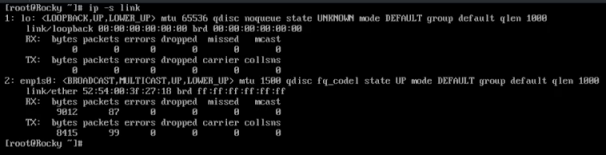
\includegraphics{1.png}
	\end{frame}
	\begin{frame}[plain]
		\item Выведите на экран информацию о текущих маршрутах:
		\\
\includegraphics{2.png}
	\end{frame}
	\begin{frame}[plain]
		\item Выведите на экран информацию о текущих назначениях адресов для сетевых интерфейсов на устройстве:
		\\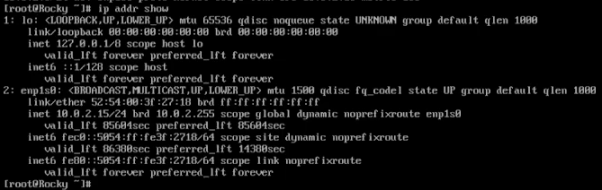
\includegraphics{3.png}
	\end{frame}
	\begin{frame}[plain]
		\item Используйте команду \texttt{ping} для проверки правильности подключения к Интернету.
		\\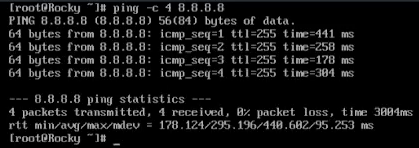
\includegraphics{4.png}
	\end{frame}
	\begin{frame}[plain]
		\item Добавьте дополнительный адрес к вашему интерфейсу:
		\\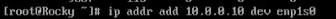
\includegraphics{5.png}
	\end{frame}
	\begin{frame}[plain]
		\item Выведите на экран список всех прослушиваемых системой портов UDP и TCP:
		\\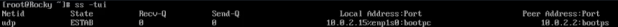
\includegraphics{6.png}
	\end{frame}
\end{itemize}

\subsection{Управление сетевыми подключениями с помощью \texttt{nmcli}}
\begin{itemize}
	\begin{frame}[plain]
		\frametitle{Управление сетевыми подключениями с помощью \texttt{nmcli}}
		\item Выведите на экран информацию о текущих соединениях:
		\\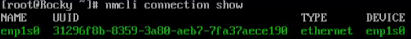
\includegraphics{7.png}
	\end{frame}
	\begin{frame}[plain]
		\item Добавьте Ethernet-соединение с именем \texttt{dhcp} к интерфейсу:
		\\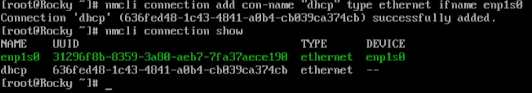
\includegraphics{8.png}
	\end{frame}
	\begin{frame}[plain]
		\item Добавьте к этому же интерфейсу Ethernet-соединение с именем \texttt{static}, статическим IPv4-адресом адаптера и статическим адресом шлюза:
		\\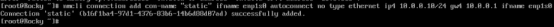
\includegraphics{9.png}
	\end{frame}
	\begin{frame}[plain]
		\item Выведите информацию о текущих соединениях:
		\\
\includegraphics{10.png}
	\end{frame}
	\begin{frame}[plain]
		\item Переключитесь на статическое соединение:
		\\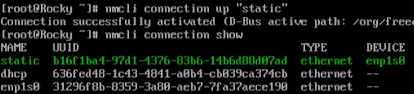
\includegraphics{11.png}
	\end{frame}
	\begin{frame}[plain]
		\item Вернитесь к соединению \texttt{dhcp}:
		\\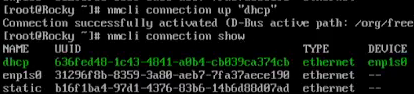
\includegraphics{12.png}
	\end{frame}
\end{itemize}

\subsection{Изменение параметров соединения с помощью \texttt{nmcli}}
\begin{itemize}
	\begin{frame}[plain]
		\frametitle{Изменение параметров соединения с помощью \texttt{nmcli}}
		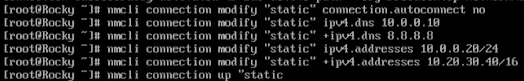
\includegraphics{13.png}
	\end{frame}
	\begin{frame}[plain]
		\item Используя \texttt{nmtui}, посмотрите настройки сети на устройстве.
		\\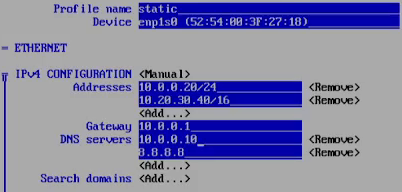
\includegraphics{14.png}
	\end{frame}
\end{itemize}

\section{Вывод}
\begin{frame}[plain]
	\frametitle{Вывод}
	В ходе выполнения данной работы я получил навыки настройки сетевых параметров системы.
\end{frame}

\end{document}
